\chapter{Data}
\label{ch:data}

\section{The National Alzheimer's Coordinating Center}

The study uses the Freeze~74 release (June 2026) of the National Alzheimer's Coordinating Center (NACC) database. NACC pools longitudinal data from Alzheimer's Disease Research Centers across the United States. Volunteers are assessed roughly once a year with the Uniform Data Set (UDS), a fixed battery of questionnaires, examinations and neuropsychological tests that every centre administers in the same way \cite{weintraub2018}. The release used here contains 217,598 visits from 57,038 participants at 46 centres, collected between June 2005 and May 2026. Participants are referred through memory clinics or volunteer directly, so the cohort is a research sample and not a population sample: at the first visit the median age is 71 years, median education is 16 years and 76\% of participants identify as White.

Access to the data is governed by the NACC data use agreement. All analysis was performed on a local machine. No participant-level value, identifier or image file name appears in this thesis, in the code repository or in any shared report; every reported number is an aggregate.

\section{Files received}

Table~\ref{tab:files} lists the ten tables in the release. Only the main clinical table and the four summary PET tables contribute model inputs; the remaining files were audited but do not supply features.

\begin{table}[H]
\centering\small
\caption{Files in the NACC release and their role in this study.}
\label{tab:files}
\begin{tabularx}{\textwidth}{@{}lrrY@{}}
\toprule
File & Rows & Participants & Role \\
\midrule
Main clinical table (\texttt{ftldlbd}) & 217,598 & 57,038 & All clinical features and the outcome \\
SCAN amyloid PET summary & 3,933 & 3,566 & Centiloids and amyloid status \\
Mixed-protocol amyloid PET summary & 2,235 & 2,073 & Same, for older scans \\
SCAN tau PET & 2,653 & 2,405 & Meta-temporal and entorhinal SUVR \\
Mixed-protocol tau PET & 671 & 616 & Same, for older scans \\
SCAN and mixed-protocol amyloid PET, regional & 6,168 & --- & Not used (tracer-specific SUVR) \\
SCAN FDG PET & 885 & 639 & Not used (about 600 linked participants) \\
SCAN PET quality-control list & 8,759 & 4,585 & Audit of the local image folders \\
CLARiTI study tracking & 857 & 776 & Not used (administrative) \\
\bottomrule
\end{tabularx}
\end{table}

In the clinical table one row is one visit; in the PET tables one row is one scan. The participant identifier is the only key shared by all tables. Because a scan is not tied to a visit number, each scan has to be matched to a visit by date (Section~\ref{sec:pettiming}).

In addition, 599 raw PET acquisitions (318 amyloid, 232 tau and 49 FDG scans from 446 participants, about 100\,GB of DICOM files) were available locally. They are used in Chapter~\ref{ch:petimages}.

\section{The clinical table}

The clinical table has 2,649 columns, but most of them are empty for most visits: modules for frontotemporal and Lewy body disease, autopsy findings, form version~4 items and free text. Only 787 columns contain data in at least 10\% of visits. From these, 114 variables were mapped by hand to a meaning, a category, a role and their own missing-value codes, following the NACC Researcher's Data Dictionary. Seventy-six of them are used to build the model inputs.

\subsection{Missing-value codes}

NACC encodes non-responses with numeric codes whose meaning depends on the variable: $-4$ marks a question that was not part of the visit, codes such as 8, 88 or 888 mark ``not applicable'', and 9, 99 or 999 mark ``unknown''. These codes cannot be removed globally. The value 88, for example, is a genuine age in 3,655 visits and a genuine diastolic pressure in 3,090 visits, but means ``never smoked'' in the years-smoked column (73,669 visits). Cleaning was therefore performed column by column from the variable map.

\subsection{Changes in the forms}

The UDS has been revised three times. The most important change for this study took place with version~3 in 2015, when the neuropsychological battery was replaced: the MMSE, Logical Memory, Digit Span and Boston Naming tests were replaced by the MoCA, Craft Story, Number Span and MINT tests. Only category fluency and the Trail Making tests are common to all versions. The same participant can therefore have different tests at different visits. Health history is also recorded on two forms: the participant-reported history (form A5) and, in version~3, the clinician-assessed conditions (form D2). Telephone visits contain no neuropsychological tests. Figure~\ref{fig:tests} shows how the availability of each test changes between versions; it is the reason the tests were converted into common domain scores (Section~\ref{sec:zscores}).

\begin{figure}[H]
\centering
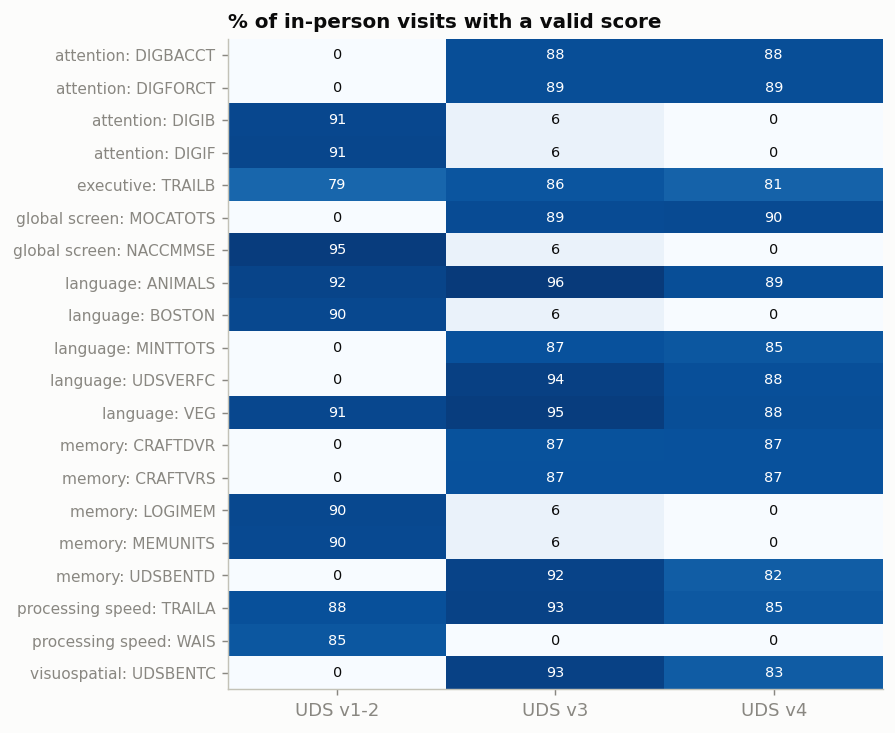
\includegraphics[width=0.8\textwidth]{03_test_availability.png}
\caption{Percentage of in-person visits with a valid score for each neuropsychological test, by UDS version. Tests of versions 1--2 and of version~3 are almost disjoint.}
\label{fig:tests}
\end{figure}


\section{Feature categories}

The variables used are grouped into five categories (Table~\ref{tab:categories}). The complete list, with source columns and value codes, is given in Appendix~A.

\begin{table}[H]
\centering\small
\caption{Feature categories, source columns and number of model features.}
\label{tab:categories}
\begin{tabularx}{\textwidth}{@{}lYr@{}}
\toprule
Category & Main source columns & Features \\
\midrule
Demographics & \texttt{NACCAGE}, \texttt{NACCSEX}, \texttt{EDUC}, \texttt{NACCNIHR}, \texttt{NACCHISP}, \texttt{NACCLIVS} & 8 \\
Cardiovascular and medical & Twelve conditions from forms A5 and D2, smoking, blood pressure, heart rate, BMI, four medication classes and the medication count & 25 \\
Cognitive tests & Twenty neuropsychological tests, the Geriatric Depression Scale and twelve NPI-Q behaviour items & 9 \\
Clinical stage & \texttt{CDRSUM}, \texttt{NACCUDSD} & 3 \\
Genetics & \texttt{NACCNE4S}, \texttt{NACCFAM} & 3 \\
PET (second-stage model only) & \texttt{CENTILOIDS}, amyloid status, meta-temporal and entorhinal tau SUVR & 4 \\
\bottomrule
\end{tabularx}
\end{table}

Four groups of variables were deliberately excluded. Autopsy findings are known only after death and would leak future information. The Functional Activities Questionnaire, the level of independence, subjective and informant-reported memory complaints and the use of Alzheimer's medication are so close to the diagnosis itself that including them would partly reproduce the clinician's decision; they were evaluated separately as a sensitivity analysis. Regional PET values were not used because they are tracer-specific and highly redundant. Form version~4 visits (3\% of visits) were excluded because they use new variable names.

\section{PET data}
\label{sec:petdata}

Amyloid PET values are available for about 5,100 participants who also appear in the clinical table, and tau PET values for 2,724. The amyloid tables provide the Centiloid value, which is comparable across tracers, and a positive or negative status assigned by the PET core. The tau tables provide standardised uptake value ratios (SUVR) in about 160 regions; the meta-temporal composite and the entorhinal cortex were retained as the standard summaries of early tau deposition. Because the two tau tracers (flortaucipir and MK-6240) give different SUVR scales, each tau value was standardised within tracer against amyloid-negative participants from the training set. Only scans that passed quality control were used.

Most PET scans are recent, so few scanned participants have three years of clinical follow-up after the scan. This limits what can be learned from PET in this cohort (Section~\ref{sec:res_pet}).
